\documentclass[border=6pt]{standalone}
\usepackage[T1]{fontenc}
\usepackage{courier}
\usepackage[scaled=0.95]{helvet}
\renewcommand{\familydefault}{\sfdefault}
\usepackage{sfmath}
\usepackage[version=4]{mhchem}
\usepackage{tikz}
\usepackage{pgfplots}
\pgfplotsset{compat=newest}
\usetikzlibrary{arrows.meta,positioning,calc,fit,backgrounds,shapes.geometric,decorations.pathreplacing,patterns}
\definecolor{ink}{HTML}{17233A}
\definecolor{inksoft}{HTML}{44506A}
\definecolor{teal}{HTML}{0E6B6B}
\definecolor{tealsoft}{HTML}{E5F0EF}
\definecolor{amber}{HTML}{B26B12}
\definecolor{ambersoft}{HTML}{FBF0DF}
\definecolor{blue}{HTML}{2F6690}
\definecolor{bluesoft}{HTML}{E3ECF4}
\definecolor{plum}{HTML}{7A4D8C}
\definecolor{plumsoft}{HTML}{EFE7F3}
\definecolor{greyc}{HTML}{8A94A3}
\definecolor{linec}{HTML}{D3DCE1}
\definecolor{oxy}{HTML}{C0392B}
\definecolor{carb}{HTML}{3B4252}
\definecolor{hyd}{HTML}{E6E9EE}
\definecolor{nit}{HTML}{2F6690}
\tikzset{
  every picture/.style={line cap=round,line join=round},
  lab/.style={font=\small, text=inksoft},
  >={Stealth[length=7pt]},
}
\pgfplotsset{
  every axis/.append style={axis line style={inksoft}, tick style={inksoft}, tick label style={font=\footnotesize, text=inksoft}, label style={font=\small, text=ink}},
}
% fragment tile: \frag{node name}{position}{colour}{content}
\newcommand{\frag}[4]{\node[draw=#3, fill=#3!12, line width=1.4pt, rounded corners=6pt, minimum width=1.25cm, minimum height=1.05cm, text=#3, font=\bfseries] (#1) at (#2) {#4};}
\newcommand{\ring}{\tikz[baseline=-0.6ex]{\draw[line width=1.1pt] (0:0.3)--(60:0.3)--(120:0.3)--(180:0.3)--(240:0.3)--(300:0.3)--cycle; \draw[line width=0.8pt] (0,0) circle (0.16);}}
\newcommand{\bond}[2]{\draw[ink, line width=2.2pt] (#1) -- (#2);}

\begin{document}
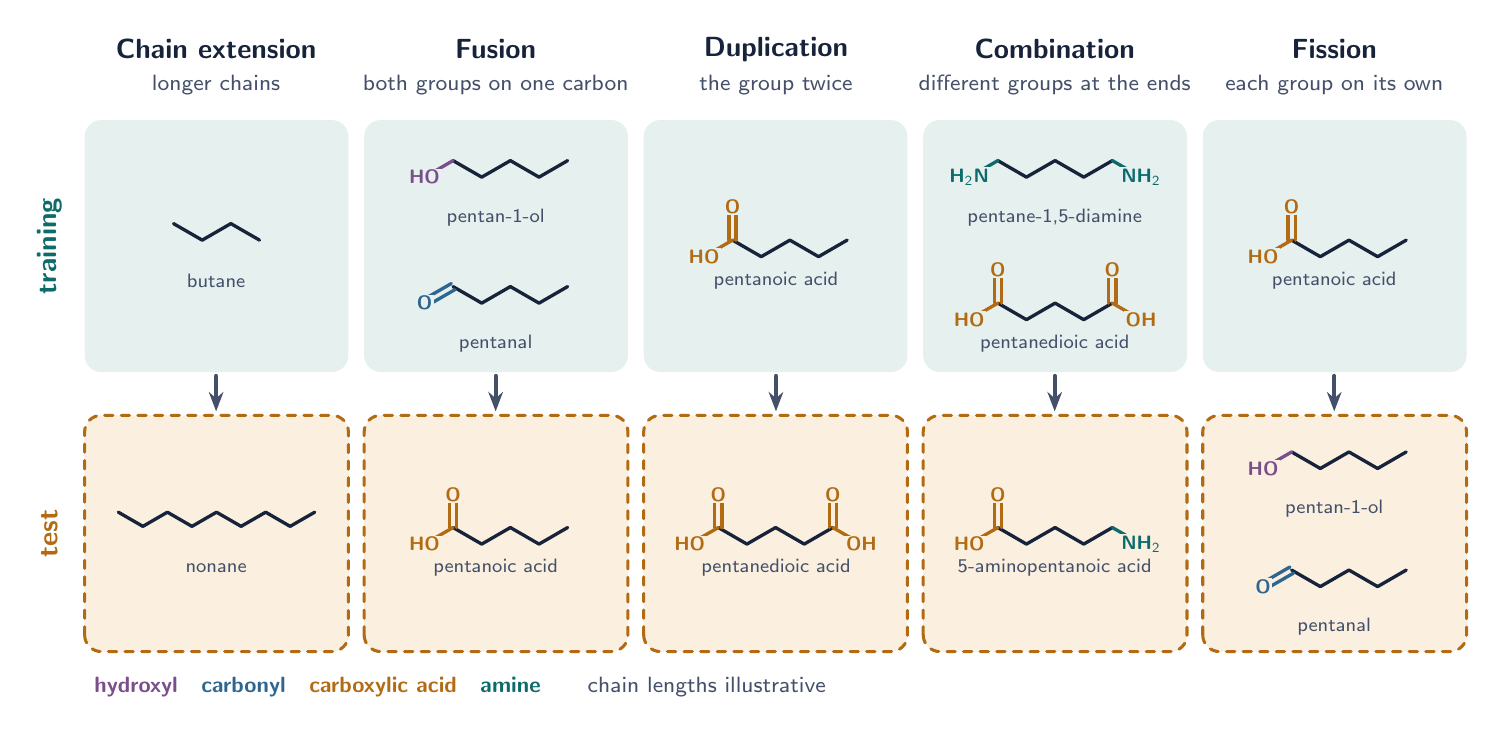
\begin{tikzpicture}
\node[font=\bfseries, text=teal, rotate=90] at (-0.35,4.60) {training};
\node[font=\bfseries, text=amber, rotate=90] at (-0.35,0.95) {test};
\node[font=\bfseries, text=ink] at (1.77,7.1) {Chain extension};
\node[font=\footnotesize, text=inksoft] at (1.77,6.65) {longer chains};
\fill[tealsoft, rounded corners=6pt] (0.10,3.00) rectangle (3.45,6.20);
\draw[amber, dashed, line width=1.1pt, fill=ambersoft, rounded corners=6pt] (0.10,-0.55) rectangle (3.45,2.45);
\draw[->, inksoft, line width=1.5pt] (1.77,2.95) -- (1.77,2.50);
\draw[ink, line width=1.2pt] (1.229,4.885) -- (1.593,4.675);
\draw[ink, line width=1.2pt] (1.593,4.675) -- (1.957,4.885);
\draw[ink, line width=1.2pt] (1.957,4.885) -- (2.321,4.675);
\node[font=\scriptsize, text=inksoft] at (1.77,4.16) {butane};
\draw[ink, line width=1.2pt] (0.528,1.220) -- (0.840,1.040);
\draw[ink, line width=1.2pt] (0.840,1.040) -- (1.151,1.220);
\draw[ink, line width=1.2pt] (1.151,1.220) -- (1.463,1.040);
\draw[ink, line width=1.2pt] (1.463,1.040) -- (1.775,1.220);
\draw[ink, line width=1.2pt] (1.775,1.220) -- (2.087,1.040);
\draw[ink, line width=1.2pt] (2.087,1.040) -- (2.399,1.220);
\draw[ink, line width=1.2pt] (2.399,1.220) -- (2.710,1.040);
\draw[ink, line width=1.2pt] (2.710,1.040) -- (3.022,1.220);
\node[font=\scriptsize, text=inksoft] at (1.77,0.51) {nonane};
\node[font=\bfseries, text=ink] at (5.32,7.1) {Fusion};
\node[font=\footnotesize, text=inksoft] at (5.32,6.65) {both groups on one carbon};
\fill[tealsoft, rounded corners=6pt] (3.65,3.00) rectangle (7.00,6.20);
\draw[amber, dashed, line width=1.1pt, fill=ambersoft, rounded corners=6pt] (3.65,-0.55) rectangle (7.00,2.45);
\draw[->, inksoft, line width=1.5pt] (5.32,2.95) -- (5.32,2.50);
\draw[ink, line width=1.2pt] (4.779,5.685) -- (5.143,5.475);
\draw[ink, line width=1.2pt] (5.143,5.475) -- (5.507,5.685);
\draw[ink, line width=1.2pt] (5.507,5.685) -- (5.871,5.475);
\draw[ink, line width=1.2pt] (5.871,5.475) -- (6.234,5.685);
\draw[plum, line width=1.2pt] (4.779,5.685) -- (4.416,5.475);
\node[font=\scriptsize\bfseries, text=plum, fill=tealsoft, inner sep=0.6pt] at (4.416,5.475) {HO};
\node[font=\scriptsize, text=inksoft] at (5.32,4.96) {pentan-1-ol};
\draw[ink, line width=1.2pt] (4.779,4.085) -- (5.143,3.875);
\draw[ink, line width=1.2pt] (5.143,3.875) -- (5.507,4.085);
\draw[ink, line width=1.2pt] (5.507,4.085) -- (5.871,3.875);
\draw[ink, line width=1.2pt] (5.871,3.875) -- (6.234,4.085);
\draw[blue, line width=1.2pt] (4.802,4.046) -- (4.438,3.836);
\draw[blue, line width=1.2pt] (4.757,4.124) -- (4.393,3.914);
\node[font=\scriptsize\bfseries, text=blue, fill=tealsoft, inner sep=0.6pt] at (4.416,3.875) {O};
\node[font=\scriptsize, text=inksoft] at (5.32,3.36) {pentanal};
\draw[ink, line width=1.2pt] (4.779,1.025) -- (5.143,0.815);
\draw[ink, line width=1.2pt] (5.143,0.815) -- (5.507,1.025);
\draw[ink, line width=1.2pt] (5.507,1.025) -- (5.871,0.815);
\draw[ink, line width=1.2pt] (5.871,0.815) -- (6.234,1.025);
\draw[amber, line width=1.2pt] (4.734,1.025) -- (4.734,1.445);
\draw[amber, line width=1.2pt] (4.824,1.025) -- (4.824,1.445);
\draw[amber, line width=1.2pt] (4.779,1.025) -- (4.416,0.815);
\node[font=\scriptsize\bfseries, text=amber, fill=ambersoft, inner sep=0.6pt] at (4.779,1.445) {O};
\node[font=\scriptsize\bfseries, text=amber, fill=ambersoft, inner sep=0.6pt] at (4.416,0.815) {HO};
\node[font=\scriptsize, text=inksoft] at (5.32,0.51) {pentanoic acid};
\node[font=\bfseries, text=ink] at (8.88,7.1) {Duplication};
\node[font=\footnotesize, text=inksoft] at (8.88,6.65) {the group twice};
\fill[tealsoft, rounded corners=6pt] (7.20,3.00) rectangle (10.55,6.20);
\draw[amber, dashed, line width=1.1pt, fill=ambersoft, rounded corners=6pt] (7.20,-0.55) rectangle (10.55,2.45);
\draw[->, inksoft, line width=1.5pt] (8.88,2.95) -- (8.88,2.50);
\draw[ink, line width=1.2pt] (8.329,4.675) -- (8.693,4.465);
\draw[ink, line width=1.2pt] (8.693,4.465) -- (9.057,4.675);
\draw[ink, line width=1.2pt] (9.057,4.675) -- (9.421,4.465);
\draw[ink, line width=1.2pt] (9.421,4.465) -- (9.784,4.675);
\draw[amber, line width=1.2pt] (8.284,4.675) -- (8.284,5.095);
\draw[amber, line width=1.2pt] (8.374,4.675) -- (8.374,5.095);
\draw[amber, line width=1.2pt] (8.329,4.675) -- (7.966,4.465);
\node[font=\scriptsize\bfseries, text=amber, fill=tealsoft, inner sep=0.6pt] at (8.329,5.095) {O};
\node[font=\scriptsize\bfseries, text=amber, fill=tealsoft, inner sep=0.6pt] at (7.966,4.465) {HO};
\node[font=\scriptsize, text=inksoft] at (8.88,4.16) {pentanoic acid};
\draw[ink, line width=1.2pt] (8.148,1.025) -- (8.511,0.815);
\draw[ink, line width=1.2pt] (8.511,0.815) -- (8.875,1.025);
\draw[ink, line width=1.2pt] (8.875,1.025) -- (9.239,0.815);
\draw[ink, line width=1.2pt] (9.239,0.815) -- (9.602,1.025);
\draw[amber, line width=1.2pt] (8.103,1.025) -- (8.103,1.445);
\draw[amber, line width=1.2pt] (8.193,1.025) -- (8.193,1.445);
\draw[amber, line width=1.2pt] (8.148,1.025) -- (7.784,0.815);
\draw[amber, line width=1.2pt] (9.557,1.025) -- (9.557,1.445);
\draw[amber, line width=1.2pt] (9.647,1.025) -- (9.647,1.445);
\draw[amber, line width=1.2pt] (9.602,1.025) -- (9.966,0.815);
\node[font=\scriptsize\bfseries, text=amber, fill=ambersoft, inner sep=0.6pt] at (8.148,1.445) {O};
\node[font=\scriptsize\bfseries, text=amber, fill=ambersoft, inner sep=0.6pt] at (7.784,0.815) {HO};
\node[font=\scriptsize\bfseries, text=amber, fill=ambersoft, inner sep=0.6pt] at (9.602,1.445) {O};
\node[font=\scriptsize\bfseries, text=amber, fill=ambersoft, inner sep=0.6pt] at (9.966,0.815) {OH};
\node[font=\scriptsize, text=inksoft] at (8.88,0.51) {pentanedioic acid};
\node[font=\bfseries, text=ink] at (12.42,7.1) {Combination};
\node[font=\footnotesize, text=inksoft] at (12.42,6.65) {different groups at the ends};
\fill[tealsoft, rounded corners=6pt] (10.75,3.00) rectangle (14.10,6.20);
\draw[amber, dashed, line width=1.1pt, fill=ambersoft, rounded corners=6pt] (10.75,-0.55) rectangle (14.10,2.45);
\draw[->, inksoft, line width=1.5pt] (12.42,2.95) -- (12.42,2.50);
\draw[ink, line width=1.2pt] (11.698,5.685) -- (12.061,5.475);
\draw[ink, line width=1.2pt] (12.061,5.475) -- (12.425,5.685);
\draw[ink, line width=1.2pt] (12.425,5.685) -- (12.789,5.475);
\draw[ink, line width=1.2pt] (12.789,5.475) -- (13.152,5.685);
\draw[teal, line width=1.2pt] (11.698,5.685) -- (11.334,5.475);
\draw[teal, line width=1.2pt] (13.152,5.685) -- (13.516,5.475);
\node[font=\scriptsize\bfseries, text=teal, fill=tealsoft, inner sep=0.6pt] at (11.334,5.475) {H$_2$N};
\node[font=\scriptsize\bfseries, text=teal, fill=tealsoft, inner sep=0.6pt] at (13.516,5.475) {NH$_2$};
\node[font=\scriptsize, text=inksoft] at (12.42,4.96) {pentane-1,5-diamine};
\draw[ink, line width=1.2pt] (11.698,3.875) -- (12.061,3.665);
\draw[ink, line width=1.2pt] (12.061,3.665) -- (12.425,3.875);
\draw[ink, line width=1.2pt] (12.425,3.875) -- (12.789,3.665);
\draw[ink, line width=1.2pt] (12.789,3.665) -- (13.152,3.875);
\draw[amber, line width=1.2pt] (11.653,3.875) -- (11.653,4.295);
\draw[amber, line width=1.2pt] (11.743,3.875) -- (11.743,4.295);
\draw[amber, line width=1.2pt] (11.698,3.875) -- (11.334,3.665);
\draw[amber, line width=1.2pt] (13.107,3.875) -- (13.107,4.295);
\draw[amber, line width=1.2pt] (13.197,3.875) -- (13.197,4.295);
\draw[amber, line width=1.2pt] (13.152,3.875) -- (13.516,3.665);
\node[font=\scriptsize\bfseries, text=amber, fill=tealsoft, inner sep=0.6pt] at (11.698,4.295) {O};
\node[font=\scriptsize\bfseries, text=amber, fill=tealsoft, inner sep=0.6pt] at (11.334,3.665) {HO};
\node[font=\scriptsize\bfseries, text=amber, fill=tealsoft, inner sep=0.6pt] at (13.152,4.295) {O};
\node[font=\scriptsize\bfseries, text=amber, fill=tealsoft, inner sep=0.6pt] at (13.516,3.665) {OH};
\node[font=\scriptsize, text=inksoft] at (12.42,3.36) {pentanedioic acid};
\draw[ink, line width=1.2pt] (11.698,1.025) -- (12.061,0.815);
\draw[ink, line width=1.2pt] (12.061,0.815) -- (12.425,1.025);
\draw[ink, line width=1.2pt] (12.425,1.025) -- (12.789,0.815);
\draw[ink, line width=1.2pt] (12.789,0.815) -- (13.152,1.025);
\draw[amber, line width=1.2pt] (11.653,1.025) -- (11.653,1.445);
\draw[amber, line width=1.2pt] (11.743,1.025) -- (11.743,1.445);
\draw[amber, line width=1.2pt] (11.698,1.025) -- (11.334,0.815);
\draw[teal, line width=1.2pt] (13.152,1.025) -- (13.516,0.815);
\node[font=\scriptsize\bfseries, text=amber, fill=ambersoft, inner sep=0.6pt] at (11.698,1.445) {O};
\node[font=\scriptsize\bfseries, text=amber, fill=ambersoft, inner sep=0.6pt] at (11.334,0.815) {HO};
\node[font=\scriptsize\bfseries, text=teal, fill=ambersoft, inner sep=0.6pt] at (13.516,0.815) {NH$_2$};
\node[font=\scriptsize, text=inksoft] at (12.42,0.51) {5-aminopentanoic acid};
\node[font=\bfseries, text=ink] at (15.97,7.1) {Fission};
\node[font=\footnotesize, text=inksoft] at (15.97,6.65) {each group on its own};
\fill[tealsoft, rounded corners=6pt] (14.30,3.00) rectangle (17.65,6.20);
\draw[amber, dashed, line width=1.1pt, fill=ambersoft, rounded corners=6pt] (14.30,-0.55) rectangle (17.65,2.45);
\draw[->, inksoft, line width=1.5pt] (15.97,2.95) -- (15.97,2.50);
\draw[ink, line width=1.2pt] (15.429,4.675) -- (15.793,4.465);
\draw[ink, line width=1.2pt] (15.793,4.465) -- (16.157,4.675);
\draw[ink, line width=1.2pt] (16.157,4.675) -- (16.521,4.465);
\draw[ink, line width=1.2pt] (16.521,4.465) -- (16.884,4.675);
\draw[amber, line width=1.2pt] (15.384,4.675) -- (15.384,5.095);
\draw[amber, line width=1.2pt] (15.474,4.675) -- (15.474,5.095);
\draw[amber, line width=1.2pt] (15.429,4.675) -- (15.066,4.465);
\node[font=\scriptsize\bfseries, text=amber, fill=tealsoft, inner sep=0.6pt] at (15.429,5.095) {O};
\node[font=\scriptsize\bfseries, text=amber, fill=tealsoft, inner sep=0.6pt] at (15.066,4.465) {HO};
\node[font=\scriptsize, text=inksoft] at (15.97,4.16) {pentanoic acid};
\draw[ink, line width=1.2pt] (15.429,1.985) -- (15.793,1.775);
\draw[ink, line width=1.2pt] (15.793,1.775) -- (16.157,1.985);
\draw[ink, line width=1.2pt] (16.157,1.985) -- (16.521,1.775);
\draw[ink, line width=1.2pt] (16.521,1.775) -- (16.884,1.985);
\draw[plum, line width=1.2pt] (15.429,1.985) -- (15.066,1.775);
\node[font=\scriptsize\bfseries, text=plum, fill=ambersoft, inner sep=0.6pt] at (15.066,1.775) {HO};
\node[font=\scriptsize, text=inksoft] at (15.97,1.26) {pentan-1-ol};
\draw[ink, line width=1.2pt] (15.429,0.485) -- (15.793,0.275);
\draw[ink, line width=1.2pt] (15.793,0.275) -- (16.157,0.485);
\draw[ink, line width=1.2pt] (16.157,0.485) -- (16.521,0.275);
\draw[ink, line width=1.2pt] (16.521,0.275) -- (16.884,0.485);
\draw[blue, line width=1.2pt] (15.452,0.446) -- (15.088,0.236);
\draw[blue, line width=1.2pt] (15.407,0.524) -- (15.043,0.314);
\node[font=\scriptsize\bfseries, text=blue, fill=ambersoft, inner sep=0.6pt] at (15.066,0.275) {O};
\node[font=\scriptsize, text=inksoft] at (15.97,-0.24) {pentanal};
\node[font=\footnotesize, text=inksoft, anchor=west] at (0.1,-1.0) {\textcolor{plum}{\textbf{hydroxyl}}\quad\textcolor{blue}{\textbf{carbonyl}}\quad\textcolor{amber}{\textbf{carboxylic acid}}\quad\textcolor{teal}{\textbf{amine}}\qquad chain lengths illustrative};
\end{tikzpicture}
\end{document}
